\documentclass[12pt,spanish]{article}
\usepackage[spanish]{babel}
\usepackage{graphicx}
\usepackage{color}
\usepackage{xcolor}
\usepackage{colortbl}
\usepackage{amsthm,thmtools}
\usepackage{multirow}
\usepackage{amsmath}
\usepackage{subcaption}
\usepackage{adjustbox}
\usepackage{multirow}
\usepackage[hidelinks]{hyperref}
\usepackage{caption}
\usepackage{amsthm}
\usepackage{multicol}
\usepackage{float}
\usepackage{amsfonts}
\usepackage{titling}
\usepackage{soul}
\usepackage{listings}
\usepackage{array}
\usepackage{tikz}
\usetikzlibrary{shapes,shapes.geometric, arrows, chains, calc,positioning,fit,decorations.pathreplacing}
\usepackage[framemethod=tikz]{mdframed}

\newcommand{\greencheck}{}%
\DeclareRobustCommand{\greencheck}{%
  \tikz\fill[scale=0.4, color=green]
  (0,.35) -- (.25,0) -- (1,.7) -- (.25,.15) -- cycle;%
}

\graphicspath{ {../img/}}
\selectlanguage{spanish}
\usepackage[utf8]{inputenc}
\usepackage{graphicx}
\usepackage[a4paper,left=3cm,right=2cm,top=2.5cm,bottom=2.5cm]{geometry}

\newenvironment{solution}{
	\par
	\textbf{Solución}
	\par
	\begin{center}
}
{
	\end{center}
}
% command \NOINDENT to be used in a group
\newcommand*\NOINDENT{\@@par   % clear parshape parameters
% fool list-awareness code (as supposedly in lstlisting, not checked)
      \@totalleftmargin\z@ \@listdepth\z@ \rightmargin\z@
}

\lstset{
  breaklines=true,
  postbreak=\mbox{\textcolor{red}{$\hookrightarrow$}\space},
}

\title{Ingeniería de Servidores}
\setlength{\droptitle}{10em}
\author{Carlos Sánchez Páez}

\makeindex
\begin{document}
\definecolor{light-gray}{gray}{0.95}
\lstset{columns=fullflexible,basicstyle=\ttfamily}
\surroundwithmdframed[
  hidealllines=true,
  backgroundcolor=light-gray,
  innerleftmargin=0pt,
  innertopmargin=0pt,
  innerbottommargin=0pt]{lstlisting}


\begin{titlepage}

 \newlength{\centeroffset}
 \setlength{\centeroffset}{-0.5\oddsidemargin}
 \addtolength{\centeroffset}{0.5\evensidemargin}
 \thispagestyle{empty}

 \noindent\hspace*{\centeroffset}
 \begin{minipage}{\textwidth}

  \centering
  
\includegraphics[width=0.9\textwidth]{logo_ugr.jpg}\\[1.4cm]

  \textsc{ \Large Ingeniería de Servidores\\[0.2cm]}
  \textsc{GRADO EN INGENIERÍA INFORMÁTICA}\\[1cm]

  {\Huge\bfseries Guión de prácticas resueltas\\}
 \end{minipage}

 \vspace{1.5cm}
 \noindent\hspace*{\centeroffset}
 \begin{minipage}{\textwidth}
  \centering

  \textbf{Autor}\\ {Carlos Sánchez Páez}\\[2.5ex]
  
\includegraphics[width=0.4\textwidth]{etsiit_logo.png}\\[0.1cm]
  \vspace{1.5cm}
  
\includegraphics[width=0.15\textwidth]{atc.jpg}\\[0.1cm]
  \vspace{1cm}
  \textsc{Escuela Técnica Superior de Ingenierías Informática y de Telecomunicación}\\
  \vspace{1cm}
  \textsc{Curso 2019-2020}
 \end{minipage}
\end{titlepage}
\thispagestyle{empty}
\newpage
\tableofcontents{}
\newpage
\listoffigures
\thispagestyle{empty}
\newpage

\section{Práctica 1: Virtualización e instalación de Sistemas Operativos}

\subsection{Sesión 1}

\subsubsection{Tipos de arquitecturas}

Un servidor es una máquina que se dedica a resolver peticiones. Hay varios tipos:
\begin{itemize}
  \item \textbf{Hosting dedicado}. Alguien monta su propio servidor y únicamente lo utiliza él.
  \item \textbf{VPS (\textit{Virtual Private Server})}. Se utiliza la virtualización para proporcionar recursos dedicados (privados) al cliente a partir de un servidor con múltiples usuarios.
  \item \textbf{\textit{Serverless}}. Se necesita un proveedor cloud (\textit{AWS, Azure, Google Cloud}...), que gestiona dinámicamente los recursos. Las aplicaciones se ejecutan al detectarse determinados eventos. Se cobra por ancho de banda utilizado, capacidad de disco duro, etc. La principal ventaja de esta arquitectura es la escalabilidad.
\end{itemize}

\begin{figure}[H]
  \centering
  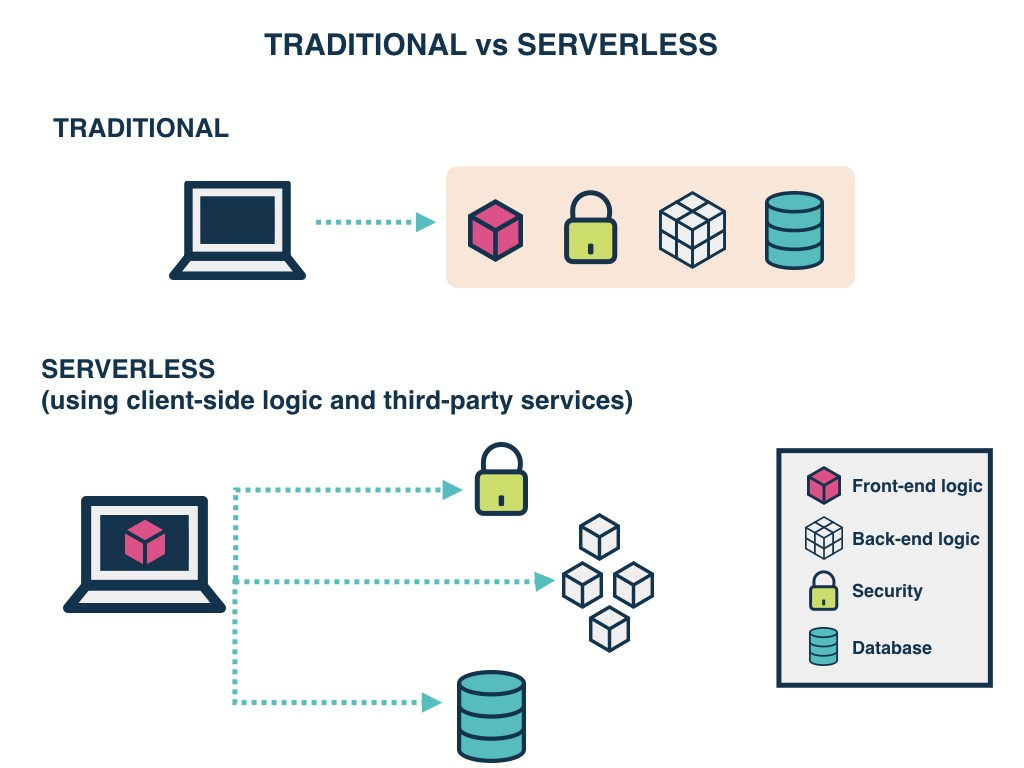
\includegraphics[width=0.55\textwidth]{serverless.jpeg}
  \vspace{0.5cm}
  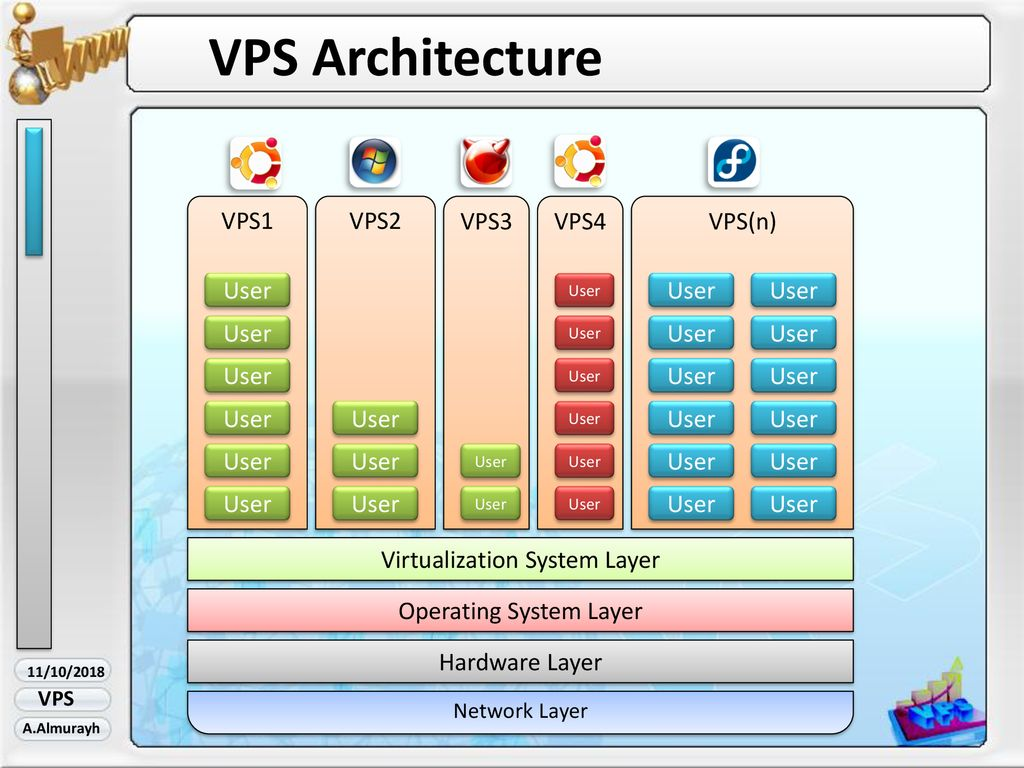
\includegraphics[width=0.55\textwidth]{vps.jpg}
  \caption{Tipos de arquitecturas de servidor}
\end{figure}

Una \textbf{máquina virtual} es aquella en la que todo su \textit{hardware} está virtualizado, es decir, compartido con el host. Las principales ventajas de las MV son precio, encapsulamiento y flexibilidad. Realmente no son más que archivos.\\

Un \textbf{contenedor} empaqueta una aplicación con sus correspondientes dependencias, consiguiendo así la máxima \textit{portabilidad}. Lo único que se necesita tener instalado en una máquina para ejecutar la aplicación es el hipervisor adecuado (por ejemplo, \textit{Docker}).\\

Un \textbf{hipervisor} es un motor que se encarga de traducir las instrucciones de una máquina virtual (o contenedor) a llamadas al sistema. Algunos ejemplos de hipervisor son \textit{VirtualBox} o \textit{VMWare}.

\begin{figure}[H]
  \centering
  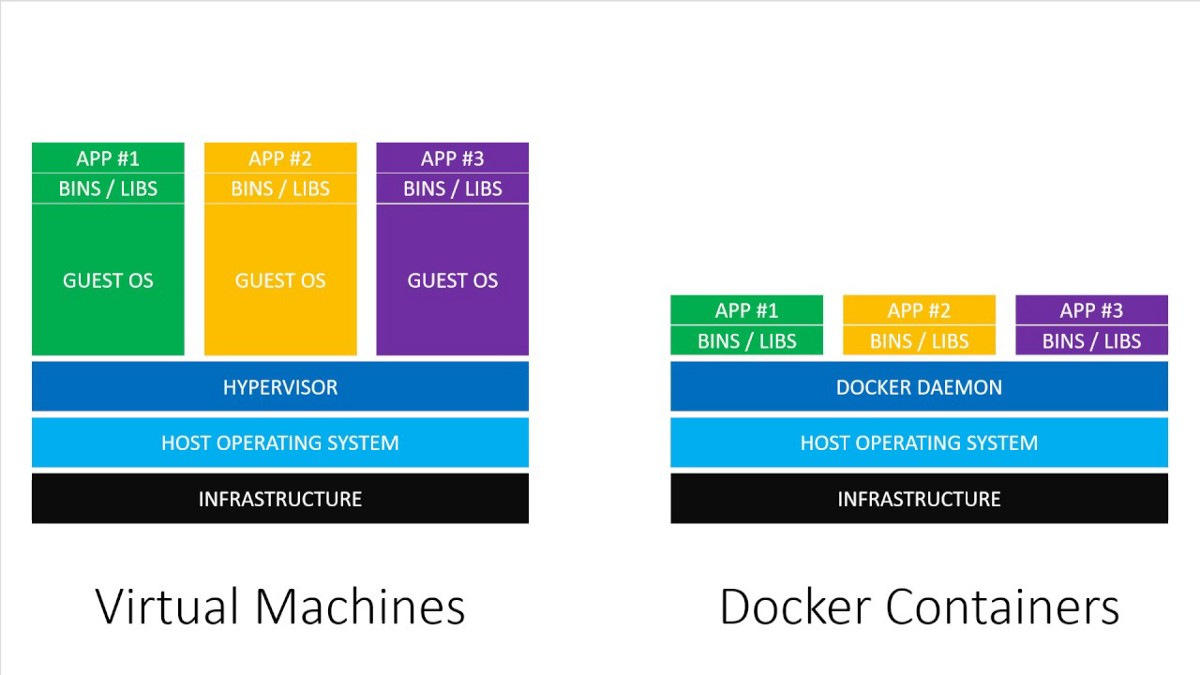
\includegraphics[width=\textwidth]{contenedor_vs_vm.jpeg}
  \caption{Diferencias entre contenedor y máquina virtual}
\end{figure}
Podríamos realizar una analogía diciendo que las máquinas virtuales son procesos (encapsulados, no pueden acceder entre ellos) y los contenedores son hebras (sí que pueden comunicarse).

\subsubsection{RAID}

RAID (\textit{\textbf{R}edundant \textbf{A}rray of \textbf{I}ndependent/\textbf{I}nexpensive} \textbf{D}isks) es una tecnología que utiliza varias unidades de almacenamiento entre las que se replican los datos. Existen varios tipos de RAID:
\begin{itemize}
  \item \textbf{RAID0}. En este modelo no hay réplica. Los datos se distribuyen equitativamente entre ambos volúmenes.
  \item \textbf{RAID1}. Los datos se copian en el otro disco (espejo).
  \item \textbf{RAID2,3,4} no se usan en la actualidad.
  \item \textbf{RAID5}. Implementa bloques de paridad como medida de redundancia. Puede fallar un disco como máximo.
  \item \textbf{RAID6}. Implementa doble paridad. Pueden fallar dos discos como máximo.
  \item \textbf{RAID0+1,RAID1+0}. Se anidan ambos tipos de RAID.
\end{itemize}

\begin{figure}[H]
  \centering
  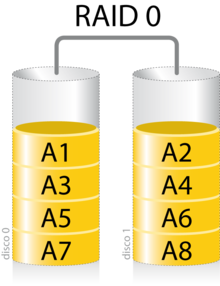
\includegraphics[width=0.2\textwidth]{raid0.png}
  \hspace{0.5cm}
  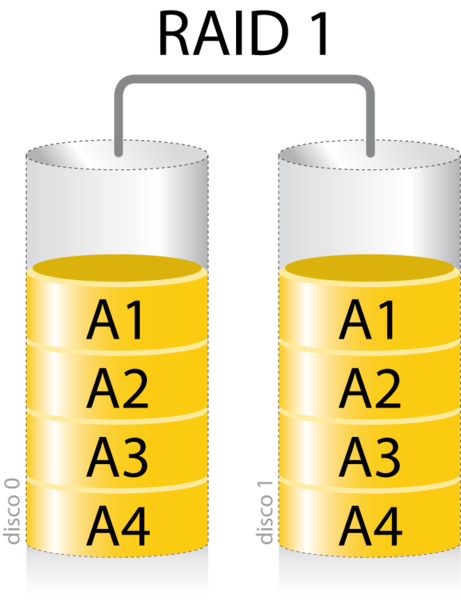
\includegraphics[width=0.2\textwidth]{raid1.png}
  \\
  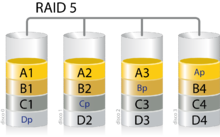
\includegraphics[width=0.4\textwidth]{raid5.png}
  \hspace{0.5cm}
  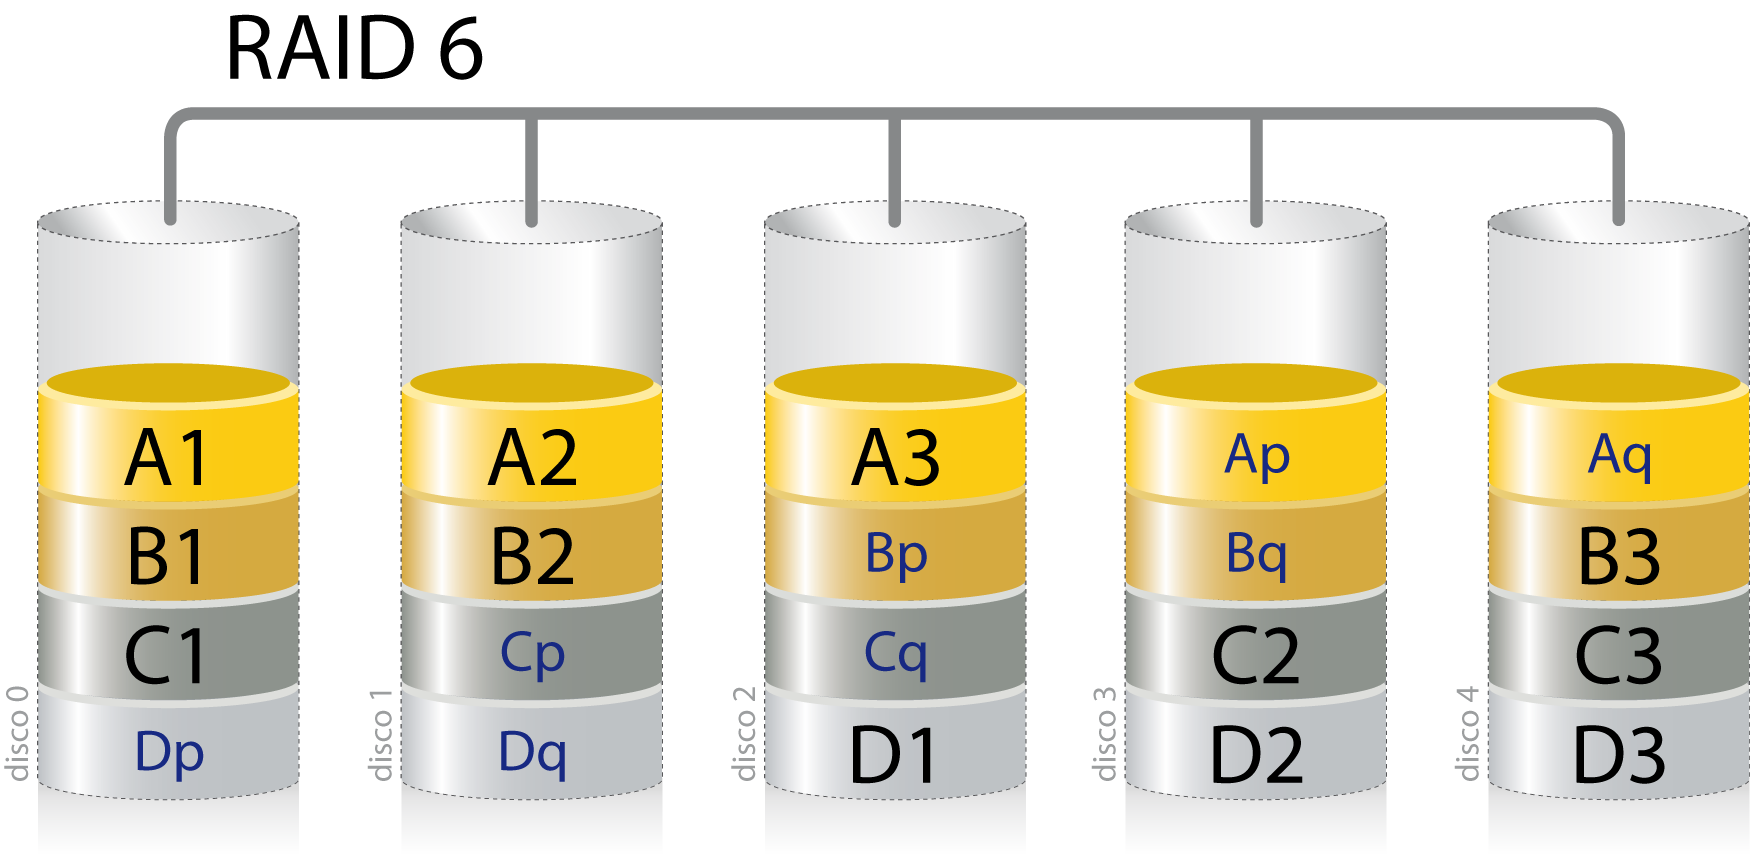
\includegraphics[width=0.4\textwidth]{raid6.png}
  \\
  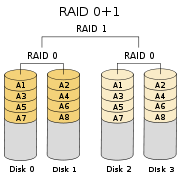
\includegraphics[width=0.4\textwidth]{raid01.png}
  \hspace{0.5cm}
  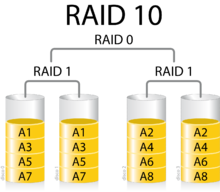
\includegraphics[width=0.4\textwidth]{raid10.png}
  \caption{Tipos de RAID}
\end{figure}

\newpage

\subsubsection{LVM}
LVM (\textit{\textbf{L}ogical \textbf{V}olume \textbf{M}anager}) provee abstracción sobre el almacenamiento físico y el sistema de ficheros. Sus mayor ventaja es la flexibilidad: podemos incorporar nuevas unidades de almacenamiento \textit{en caliente} (sin parar el sistema) de forma sencilla. LVM está compuesto por:
\begin{itemize}
  \item Volumen físico (\textit{Physical Volume}, \textbf{PV}). Es un dispositivo de almacenamiento (HDD, partición, RAID...).
  \item Grupo de volúmenes (\textit{Volume Group}, \textbf{VG}). Es el centro de LVM. Está formado por uno o más PV. Para aumentar su espacio sólo hay que añadir más volúmenes físicos, siendo esto transparente para los sistemas de archivos, procesos o usuarios.
  \item Volumen lógico (\textit{Logical Volume}, \textbf{LV}). Es el ``producto final'', es decir, dispositivos que usaremos para crear sistemas de ficheros. Podríamos decir que son las particiones.
\end{itemize}

\begin{figure}[H]
  \centering
  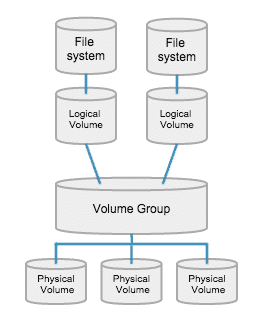
\includegraphics[width=0.65\textwidth]{lvm.png}
  \caption{Arquitectura LVM}
\end{figure}
\newpage
La estructura a crear es la siguiente:
\begin{figure}[H]
	\centering
	\begin{tikzpicture}[arrow/.style = {thick,-stealth}, node distance=2cm]
		\tikzset{set/.style={draw,rectangle,inner sep=0pt,align=center}}

		% HDDs
		\node[fit={(-1,0) (2,1)}, inner sep=0pt, draw=black, thick, text centered,fill=blue!20] (sda) {sda};

		\node[fit={(3,0) (6,1)}, inner sep=0pt, draw=black, thick, text centered,fill=blue!30] (sdb) {sdb};


		% PVs
		\node[above of=sdb, inner sep=0pt, draw=black, thick, text centered,fill=green!20, minimum width = 2cm, minimum height=1cm] (sdbpv) {sdb};

		\node[above of=sda, inner sep=0pt, draw=black, thick, text centered,fill=green!20, minimum width = 2cm, minimum height=1cm] (sdapv) {sda};

		% VGs
		\coordinate (CENTER) at ($(sdapv)!0.5!(sdbpv)$);
		\node[ellipse,above of=CENTER, inner sep=0pt, draw=black, thick, text centered, minimum size = 1cm,fill=yellow!20] (cl) {Servidor};

		% LVs
		\node[ellipse,above of=cl, inner sep=0pt, draw=black, thick, text centered, minimum size = 1cm,fill=brown!25] (raizlv) {raíz};

		\node[ellipse,left of=raizlv, inner sep=0pt, draw=black, thick, text centered, minimum size = 1cm,fill=brown!25] (arranquelv) {arranque};

		\node[ellipse,right of=raizlv, inner sep=0pt, draw=black, thick, text centered, minimum size = 1cm,fill=brown!25] (swaplv) {swap};

		\node[ellipse,right of=swaplv, inner sep=0pt, draw=black, thick, text centered, minimum size = 1cm,fill=brown!25] (hogarlv) {hogar};


		% FS
		\node[diamond, above of=swaplv,inner sep=0pt, draw=black, thick, text centered, minimum size = 1cm,fill=red!20] (swapfs) {swap};

		\node[diamond, above of=raizlv,inner sep=0pt, draw=black, thick, text centered, minimum size = 1cm,fill=red!20] (raizfs) {/};

		\node[diamond, above of=arranquelv,inner sep=0pt, draw=black, thick, text centered, minimum size = 1cm,fill=red!20] (arranquefs) {/boot};

		\node[diamond, above of=hogarlv,inner sep=0pt, draw=black, thick, text centered, minimum size = 1cm,fill=red!20] (hogarfs) {/home};

		% Curly braces
		\draw [decorate,decoration={brace,amplitude=10pt, raise=2.5pt, mirror}]	(8.5,0) -- (8.5,1) node [black,midway,xshift=1cm] {\footnotesize HDD};

		\draw [decorate,decoration={brace,amplitude=10pt, raise=2.5pt, mirror}]	(8.5,2) -- (8.5,3) node [black,midway,xshift=1cm] {\footnotesize PV};

		\draw [decorate,decoration={brace,amplitude=10pt, raise=2.5pt, mirror}]	(8.5,4) -- (8.5,5) node [black,midway,xshift=1cm] {\footnotesize VG};

		\draw [decorate,decoration={brace,amplitude=10pt, raise=2.5pt, mirror}]	(8.5,6) -- (8.5,7) node [black,midway,xshift=1cm] {\footnotesize LV};

		\draw [decorate,decoration={brace,amplitude=10pt, raise=2.5pt, mirror}]	(8.5,7.5) -- (8.5,9) node [black,midway,xshift=1cm] {\footnotesize FS};

		% Arrows

		\draw [arrow] (sda) -- (sdapv);
		\draw [arrow] (sdb) -- (sdbpv);
		\draw [arrow] (sdapv) -- (cl);
		\draw [arrow] (sdbpv) -- (cl);
		\draw [arrow] (cl) -- (arranquelv);
		\draw [arrow] (cl) -- (raizlv);
		\draw [arrow] (cl) -- (hogarlv);
		\draw [arrow] (cl) -- (swaplv);
		\draw [arrow] (arranquelv) -- (arranquefs);
		\draw [arrow] (raizlv) -- (raizfs);
		\draw [arrow] (hogarlv) -- (hogarfs);
		\draw [arrow] (swaplv) -- (swapfs);


	\end{tikzpicture}
\end{figure}

\subsubsection{Instalación de Ubuntu Server con RAID1}
\begin{enumerate}
  \item Descargamos la ISO desde \href{http://atcproyectos.ugr.es/esriie/ubuntu-16.04.5-server-amd64.iso}{aquí}.
  \item Creamos una máquina virtual con 1024MB RAM y dos discos duros VDI reservados dinámicamente de 10GB cada uno. Por último, montamos la ISO en el controlador IDE.
  \item  Arrancamos la máquina, marcamos idioma español y procedemos a la instalación.
  \item Elegimos España y la distribución de teclado Spanish/Spanish.
	\item Dejamos el nombre de la máquina en ``ubuntu'' y establecemos el nombre de usuario con nuestras iniciales. La clave será \textit{practicas,ISE}.
	\item No ciframos la carpeta personal, ya que usaremos FDE (\textit{Full Disk Encryption}).
	\item Aceptamos la zona horaria propuesta.
	\item Elegimos particionado manual.
	\item Damos Enter en ambos discos para crear las tablas de particiones.
	\item Comenzamos configurando RAID (\textit{Configurar RAID por software}).
	\item Creamos dispositivo MD (\textit{Multiple Devices}), elegimos RAID1, establecemos 2 discos en uso y 0 vacíos, los seleccionamos y damos a terminar.
	\item Pasamos a configurar LVM (\textit{Configurar el Gestor de Volúmenes Lógicos (LVM)}).
	\item Creamos el grupo de volúmenes, con nombre \textit{Servidor} y elegimos \textit{/dev/md0}.
	\item Creamos ahora los volúmenes lógicos sobre Servidor (\textit{swap} (1024MB),\textit{arranque} (200MB),\textit{hogar} (800MB) y \textit{raíz} (resto)). Por último, damos a terminar.
	\item Pasamos a la configuración del cifrado (\textit{Configurar los volúmenes cifrados}).
	\item Damos a \textit{Create encrypted volumes} y seleccionamos todos menos \textit{arranque} (si lo encriptamos no podremos arrancar el sistema).
	\item Mantenemos los parámetros predeterminados, por lo que elegimos \textit{Se ha terminado de definir la partición} en todos los casos.
	\item Damos \textit{Sí} a mantener la distribución existente, \textit{Finish} y establecemos la clave \textit{practicas,ISE} en todos los volúmenes.
	\item Por último, vamos a formatear los volúmenes y asignar los puntos de montaje. Para ello, elegimos las particiones (marcadas con el símbolo \textbf{\#}) \textit{arranque}, \textit{hogar} y \textit{raíz}. Seleccionamos \textit{Utilizar como: sistema de ficheros ext4 transaccional} y asignamos los puntos de montaje \textit{/boot}, \textit{/home} y \textit{/} respectivamente.
	\item Para la partición \textit{swap}, elegimos \textit{Utilizar como: área de intercambio}.
	\item Finalizamos el particionado y esperamos.
	\item Dejamos en blanco el campo de proxy y elegimos la opción \textit{Sin actualizaciones automáticas}, ya que queremos mantener el control total sobre el sistema.
	\item Dejamos seleccionado \textit{Standard system utilities} y pulsamos Enter.
	\item Instalamos en cargador de arranque en \textit{/dev/sda}.
	\item Una vez que el sistema esté instalado, iniciamos sesión y desbloqueamos los volúmenes cifrados.
	\item Pasamos ahora a instalar \textit{GRUB} en el otro disco. Para ello ejecutamos:
	\begin{lstlisting}
		$> sudo grub install /dev/sdb
	\end{lstlisting}
	\item Para finalizar, tomamos una instantánea de la máquina para poder volver a este estado (Instantánea $\implies$ Tomar)

\end{enumerate}

\subsubsection{Configuración de red de Ubuntu Server}

Necesitamos configurar la red de forma que las máquinas puedan comunicarse entre sí,con el \textit{host} y con el exterior. Para ello, seguiremos los siguientes pasos:
\begin{enumerate}
	\item Crear una red sólo-anfitrión.
	\begin{enumerate}
		\item En VirtualBox (¡no en la máquina!) damos a Archivo-Administrador de red anfitrión.
		\item Seleccionamos Crear y comprobamos que la IPv4a sea 192.168.56.1. En caso contrario, la modificamos.
		\item En la configuración de la máquina virtual Ubuntu, habilitamos el adaptador 2 (conectado a adaptador sólo-anfitrión)
	\end{enumerate}
	\item Añadir la interfaz y activarla.
	\begin{enumerate}
		\item Arrancamos la máquina.
		\item Editamos el archivo de interfaces mediante \textit{sudo nano /etc/network/interfaces}.
		\item Añadimos el siguiente código:
		\begin{lstlisting}
			# Host-only interface
			auto enp0s8
			iface enp0s8 inet static
			address 192.168.56.105
		\end{lstlisting}
		\item Salimos y guardamos.
		\item Activamos la interfaz con \textit{sudo ifup enp0s8}.
		\item Ejecutamos \textit{ip addr} y comprobamos que la interfaz tiene asignada la IP que configuramos (192.168.56.105).
	\end{enumerate}
	\item Comprobar que funciona.
		\begin{enumerate}
			\item Desde nuestro host, abrimos una terminal y ejecutamos \textit{ping 192.168.56.105 -c 5}. Deberíamos recibir las 5 respuestas.
			\item Desde la máquina virtual ejecutamos \textit{ping 192.168.56.1 -c 5}. Deberíamos recibir las 5 respuestas.
		\end{enumerate}
\end{enumerate}

\subsection{Sesión 2}
\subsubsection{Instalación de CentOS}
\begin{enumerate}
	\item Descargamos la ISO desde \href{http://atcproyectos.ugr.es/esriie/ubuntu-16.04.5-server-amd64.iso}{este enlace}.
	\item Creamos una máquina virtual con 1024MB de RAM y un disco duro de 10GB (elegimos la opción \textit{Fedora 64bits}). Por último, montamos la ISO.
	\item Seleccionamos \textit{Install CentOS Linux}.
	\item Elegimos Español (España).
	\item En \textit{Destino de la instalación} elegimos el único disco disponible y damos a \textit{Listo} y a \textit{Empezar instalación}.
	\item Creamos el usuario (iniciales como usuario y \textit{practicas,ISE} como clave). Establecemos también la contraseña del \textit{root} (\textit{practicas,ISE}).
	\item Tomamos una instantánea de la máquina.
\end{enumerate}

La temática de esta sesión es la siguiente: necesitamos espacio en \textit{/var} pero no tenemos suficiente. Para dar solución a ello, tendremos que seguir estos pasos:
\begin{enumerate}
	\item Añadir el disco a la máquina.
	\item Configurar el disco mediante \textit{LVM} y darle formato.
	\item Copiar los datos de \textit{/var} al nuevo volumen.
	\item Indicar al SO que monte el nuevo volumen en \textit{/var}.
	\item Borrar los datos antiguos de \textit{/var} (en la vida real ésto se haría un tiempo prudencial después para poder disponer de un backup.)
\end{enumerate}

Básicamente, tenemos que pasar del esquema actual:
\begin{figure}[H]
	\centering
	\begin{tikzpicture}[arrow/.style = {thick,-stealth}, node distance=2cm]
		\tikzset{set/.style={draw,rectangle,inner sep=0pt,align=center}}

		% HDDs
		\node[fit={(-1,0) (2,1)}, inner sep=0pt, draw=black, thick, text centered,fill=blue!20] (sda1) {sda1};

		\node[fit={(2,0) (5,1)}, inner sep=0pt, draw=black, thick, text centered,fill=blue!30] (sda2) {sda2};


		% PVs
		\node[above of=sda2, inner sep=0pt, draw=black, thick, text centered,fill=green!20, minimum width = 2cm, minimum height=1cm] (sda2pv) {sda2};

		% VGs
		\node[ellipse,above of=sda2pv, inner sep=0pt, draw=black, thick, text centered, minimum size = 1cm,fill=yellow!20] (cl) {cl};

		% LVs
		\node[ellipse,above left of=cl, inner sep=0pt, draw=black, thick, text centered, minimum size = 1cm,fill=brown!25] (/lv) {root};

		\node[ellipse,above right of=cl, inner sep=0pt, draw=black, thick, text centered, minimum size = 1cm,fill=brown!25] (swaplv) {swap};


		% FS
		\node[diamond, above of=swaplv,inner sep=0pt, draw=black, thick, text centered, minimum size = 1cm,fill=red!20] (swapfs) {swap};

		\node[diamond, above of=/lv,inner sep=0pt, draw=black, thick, text centered, minimum size = 1cm,fill=red!20] (/fs) {/};

		\node[diamond, above of=sda1,inner sep=0pt, draw=black, thick, text centered, minimum size = 1cm,fill=red!20, node distance=7.3cm] (bootfs) {/boot};


		% Curly braces
		\draw [decorate,decoration={brace,amplitude=10pt, raise=2.5pt, mirror}]	(6,0) -- (6,1) node [black,midway,xshift=1cm] {\footnotesize HDD};

		\draw [decorate,decoration={brace,amplitude=10pt, raise=2.5pt, mirror}]	(6,2) -- (6,3) node [black,midway,xshift=1cm] {\footnotesize PV};

		\draw [decorate,decoration={brace,amplitude=10pt, raise=2.5pt, mirror}]	(6,4) -- (6,5) node [black,midway,xshift=1cm] {\footnotesize VG};

		\draw [decorate,decoration={brace,amplitude=10pt, raise=2.5pt, mirror}]	(6,5.5) -- (6,6.5) node [black,midway,xshift=1cm] {\footnotesize LV};

		\draw [decorate,decoration={brace,amplitude=10pt, raise=2.5pt, mirror}]	(6,7) -- (6,8.8) node [black,midway,xshift=1cm] {\footnotesize FS};

		% Arrows

		\draw [arrow] (sda2) -- (sda2pv);
		\draw [arrow] (sda2pv) -- (cl);
		\draw [arrow] (cl) -- (/lv);
		\draw [arrow] (cl) -- (swaplv);
		\draw [arrow] (/lv) -- (/fs);
		\draw [arrow] (sda1) -- (bootfs);
		\draw [arrow] (swaplv) -- (swapfs);

	\end{tikzpicture}
\end{figure}

Al siguiente:

\begin{figure}[H]
	\centering
	\begin{tikzpicture}[arrow/.style = {thick,-stealth}, node distance=2cm]
		\tikzset{set/.style={draw,rectangle,inner sep=0pt,align=center}}

		% HDDs
		\node[fit={(-1,0) (2,1)}, inner sep=0pt, draw=black, thick, text centered,fill=blue!20] (sda1) {sda1};

		\node[fit={(2,0) (5,1)}, inner sep=0pt, draw=black, thick, text centered,fill=blue!30] (sda2) {sda2};

		\node[fit={(6,0) (8,1)}, inner sep=0pt, draw=black, thick, text centered, fill=blue!30] (sdb) {sdb};

		% PVs
		\node[above of=sda2, inner sep=0pt, draw=black, thick, text centered,fill=green!20, minimum width = 2cm, minimum height=1cm] (sda2pv) {sda2};

		\node[above of=sdb, inner sep=0pt, draw=black, thick, text centered,,fill=green!20, minimum width = 2cm, minimum height=1cm] (sdbpv) {sdb};

		% VGs
		\node[ellipse,above right of=sda2pv, inner sep=0pt, draw=black, thick, text centered, minimum size = 1cm,fill=yellow!20] (cl) {cl};

		% LVs
		\node[ellipse,above left of=cl, inner sep=0pt, draw=black, thick, text centered, minimum size = 1cm,fill=brown!25] (/lv) {root};

		\node[ellipse,above of=cl, inner sep=0pt, draw=black, thick, text centered, minimum size = 1cm,fill=brown!25] (swaplv) {swap};

		\node[circle, above right of=cl, inner sep=0pt, draw=black, thick, text centered, minimum size = 1cm,fill=brown!25] (varlv) {/var};

		% FS
		\node[diamond, above of=swaplv,inner sep=0pt, draw=black, thick, text centered, minimum size = 1cm,fill=red!20] (swapfs) {swap};

		\node[diamond, above of=/lv,inner sep=0pt, draw=black, thick, text centered, minimum size = 1cm,fill=red!20] (/fs) {/};

		\node[diamond, above of=sda1,inner sep=0pt, draw=black, thick, text centered, minimum size = 1cm,fill=red!20, node distance=6.5cm] (bootfs) {/boot};

		\node[diamond, above of=varlv,inner sep=0pt, draw=black, thick, text centered, minimum size = 1cm,fill=red!20] (varfs) {/var};

		% Curly braces
		\draw [decorate,decoration={brace,amplitude=10pt, raise=2.5pt, mirror}]	(9,0) -- (9,1) node [black,midway,xshift=1cm] {\footnotesize HDD};

		\draw [decorate,decoration={brace,amplitude=10pt, raise=2.5pt, mirror}]	(9,2) -- (9,3) node [black,midway,xshift=1cm] {\footnotesize PV};

		\draw [decorate,decoration={brace,amplitude=10pt, raise=2.5pt, mirror}]	(9,3.5) -- (9,4.5) node [black,midway,xshift=1cm] {\footnotesize VG};

		\draw [decorate,decoration={brace,amplitude=10pt, raise=2.5pt, mirror}]	(9,4.75) -- (9,6) node [black,midway,xshift=1cm] {\footnotesize LV};

		\draw [decorate,decoration={brace,amplitude=10pt, raise=2.5pt, mirror}]	(9,6.5) -- (9,8.5) node [black,midway,xshift=1cm] {\footnotesize FS};

		% Arrows

		\draw [arrow] (sda2) -- (sda2pv);
		\draw [arrow] (sdb) -- (sdbpv);
		\draw [arrow] (sdbpv) -- (cl);
		\draw [arrow] (sda2pv) -- (cl);
		\draw [arrow] (cl) -- (/lv);
		\draw [arrow] (cl) -- (swaplv);
		\draw [arrow] (/lv) -- (/fs);
		\draw [arrow] (sda1) -- (bootfs);
		\draw [arrow] (swaplv) -- (swapfs);
		\draw [arrow] (cl) -- (varlv);
		\draw [arrow] (varlv) -- (varfs);

	\end{tikzpicture}
\end{figure}

\paragraph{Añadir el disco a la máquina}
Mediante el administrador de VirtualBox añadimos un nuevo disco (VDI, 10GB, reserva dinámica) a nuestra instancia.
\paragraph{Configurar el disco mediante \textit{LVM} y darle formato}
\begin{enumerate}
	\item Arrancamos la máquina.
	\item Comprobamos que el disco efectivamente ha sido detectado mediante \textit{lsblk}(\textbf{L}i\textbf{S}t \textbf{BL}oc\textbf{K} devices). Deberíamos ver el nuevo dispositivo \textit{/dev/sdb}. Podemos apreciar también aquí que \emph{CentOS} usa \textit{LVM} de forma nativa, bajo un grupo de volúmenes llamado \textit{cl}. También podemos ver como \textit{/boot} está sobredimensionado. Esto se hace para poder tener un backup del kernel antiguo en caso de que deba actualizarse.
	\item Como vamos a modificar elementos del sistema, nos logueamos como superusuario:
	\begin{lstlisting}
		$> su
	\end{lstlisting}
	\item Podemos ver los detalles de \textit{LVM} mediante los comandos \textit{lvdisplay} (\textit{\textbf{L}ogical \textbf{V}olume Display}), \textit{vgdisplay} (\textit{\textbf{V}olume \textbf{G}roup Display}) o \textit{pvdisplay} (\textit{\textbf{P}hysical \textbf{V}olume Display}).
	\item Creamos el volumen físico:
	\begin{lstlisting}
		#> pvcreate /dev/sdb
	\end{lstlisting}
	Podemos leer en el \textit{man} que podemos ejecutar el comando tanto en discos duros como en particiones. Comprobamos que se ha creado mediante \textit{pvdisplay}.
	\item Ahora debemos añadir el volumen físico al grupo de volúmenes existente (\textit{cl}). Para ello, ejecutamos
	\begin{lstlisting}
		#> vgextend cl /dev/sdb
	\end{lstlisting}
	Comprobamos que ha ido bien mediante \textit{vgdisplay}.
	\item Por último, debemos crear el volumen lógico. Para ello, ejecutamos el siguiente comando:
	\begin{lstlisting}
		#> lvcreate -L 5G -n newvar cl
	\end{lstlisting}
	Donde:
	\begin{itemize}
		\item -L indica el tamaño del volumen.
		\item -n indica el nombre del volumen.
	\end{itemize}
	Para finalizar, comprobamos que ha ido bien mediante \textit{lvdisplay}.
\end{enumerate}
En este momento \textit{LVM} ha sido configurado completamente.
\paragraph{Dar formato al nuevo volumen}
\begin{enumerate}
	\item Debemos comenzar creando un sistema de archivos en nuestro volumen lógico. Pero primero debemos ver cuál es el punto de montaje del mismo mediante \textit{lvdisplay} (campo \textit{LV Path}).
	\item Ahora ejecutamos el comando para crear el sistema de archivos:
	\begin{lstlisting}
		#> mkfs -t ext4 /dev/cl/newvar
	\end{lstlisting}
\end{enumerate}

\paragraph{Copiar los datos de \textit{/var} al nuevo volumen}
\begin{enumerate}
	\item Lo primero que debemos hacer es montar el volumen. Para ello ejecutamos
	\begin{lstlisting}
		#> mkdir /mnt/newvar
		#> mount /dev/cl/newvar /mnt/newvar
	\end{lstlisting}
	Comprobamos con \textit{mount}.
	\item Ahora debemos plantearnos lo siguiente: la copia debe realizarse de forma \emph{atómica}, es decir, nadie puede modificar ningún archivo, ya que esto generaría inconsistencias. Para ello, accedemos al modo de mantenimiento:
	\begin{lstlisting}
		#> systemctl isolate runlevel1.target
	\end{lstlisting}
	Introducimos de nuevo la clave del \textit{root}.
	\item Realizamos la copia de los ficheros:
	\begin{lstlisting}
		#> cp -a /var/. /mnt/newvar
	\end{lstlisting}
	Donde:
	\begin{itemize}
		\item -a indica que se deben copiar los archivos recursivamente, manteniendo enlaces y preservando el contexto. El contexto está compuesto por políticas de seguridad de \textit{SELinux} (\textit{\textbf{S}ecurity \textbf{E}nhanced Linux}) que controlan el acceso a recursos de los procesos.
		\item /var/. indica todos los archivos (incluidos los ocultos).
	\end{itemize}
	Comprobamos mediante \textit{ls -ahZ} sobre \textit{/var} y \textit{mnt/newvar}
\end{enumerate}

\paragraph{Indicarle al SO que monte el nuevo volumen en \textit{/var}}
\begin{enumerate}
	\item Abrimos el editor de texto sobre \textit{/etc/fstab}
	\begin{lstlisting}
		#> vi /etc/fstab
	\end{lstlisting}
	\item Pulsamos \textit{i} para acceder al modo de inserción y añadimos la siguiente línea:
	\begin{lstlisting}
		/dev/mapper/cl-newvar /var ext4 defaults 0 0
	\end{lstlisting}
	\item Salimos de vi (ESC, escribimos \textit{:wq} y Enter).
	\item Desmontamos el nuevo volumen:
	\begin{lstlisting}
		#> umount /mnt/newvar
	\end{lstlisting}
	\item Montamos los sistemas de archivos de \textit{/etc/fstab}:
	\begin{lstlisting}
		#> mount -a
	\end{lstlisting}
	Comprobamos ejecutando \textit{mount}.
\end{enumerate}

\paragraph{Borrar los datos antiguos de \textit{/var}}
Actualmente no tenemos acceso al antiguo \textit{/var} (el que tenemos montado actualmente es el nuevo).
\begin{enumerate}
	\item Comenzamos desmontando \textit{/var}:
	\begin{lstlisting}
		#> umount /dev/mapper/cl-newvar
	\end{lstlisting}
	\item Cambiamos el nombre de \textit{/var}:
	\begin{lstlisting}
		#> mv /var /var_old
	\end{lstlisting}
	\item Creamos \textit{/var} para que se pueda montar:
	\begin{lstlisting}
		#> mkdir /var
	\end{lstlisting}
	\item Restauramos el contexto de \textit{/var}:
	\begin{lstlisting}
		#> restorecon /var
	\end{lstlisting}
	\item Montamos la nueva partición \textit{/var}:
	\begin{lstlisting}
		#> mount -a
	\end{lstlisting}
	\item Salimos del modo de seguridad:
	\begin{lstlisting}
		#> systemctl isolate default
	\end{lstlisting}
	\item Eliminamos los archivos antiguos:
	\begin{lstlisting}
		#> rm -rf /var_old
	\end{lstlisting}
	\item Como de costumbre, tomamos la instantánea.
\end{enumerate}


\subsection{Sesión 3}

Deberemos partir de una instalación fresca de CentOS (restauramos la instantánea correspondiente). El objetivo es configurar un RAID1 con cifrado. El esquema sería el siguiente:

\begin{figure}[H]
	\centering
	\begin{tikzpicture}[arrow/.style = {thick,-stealth}, node distance=2cm]
		\tikzset{set/.style={draw,rectangle,inner sep=0pt,align=center}}

		% HDDs
		\node[fit={(-1,0) (2,1)}, inner sep=0pt, draw=black, thick, text centered,fill=blue!20] (sda1) {sda1};

		\node[fit={(2,0) (5,1)}, inner sep=0pt, draw=black, thick, text centered,fill=blue!30] (sda2) {sda2};

		\node[fit={(6,0) (9,1)}, inner sep=0pt, draw=black, thick, text centered,fill=blue!40] (sdb) {sdb};

		\node[fit={(10,0) (13,1)}, inner sep=0pt, draw=black, thick, text centered,fill=blue!40] (sdc) {sdc};

		% PVs
		\coordinate (CENTER) at ($(sdb)!0.5!(sdc)$);

		\node[above of=CENTER, inner sep=0pt, draw=black, thick, text centered,fill=green!20, minimum width = 2cm, minimum height=1cm] (md0) {md0};

		\node[above of=sda2, inner sep=0pt, draw=black, thick, text centered,fill=green!20, minimum width = 2cm, minimum height=1cm] (sda2pv) {sda2};

		% VGs
		\node[ellipse,above of=sda2pv, inner sep=0pt, draw=black, thick, text centered, minimum size = 1cm,fill=yellow!20] (cl) {cl};

		\node[ellipse,above of=md0, inner sep=0pt, draw=black, thick, text centered, minimum size = 1cm,fill=yellow!20] (pmraid1) {pmraid1};

		% LVs
		\node[ellipse,above left of=cl, inner sep=0pt, draw=black, thick, text centered, minimum size = 1cm,fill=brown!25] (/lv) {root};

		\node[ellipse,above right of=cl, inner sep=0pt, draw=black, thick, text centered, minimum size = 1cm,fill=brown!25] (swaplv) {swap};

		\node[ellipse,above of=pmraid1, inner sep=0pt, draw=black, thick, text centered, minimum size = 1cm,fill=brown!25, node distance = 1.5cm] (newvar) {newvar};

		% CRYPT
		\node[rectangle, above of=newvar,inner sep=0pt, draw=black, thick, text centered, minimum size = 1cm, minimum width=4.5cm,fill=violet!20] (newvarcrypt) {pmraid1-newvar\_crypt};

		% FS
		\node[diamond, above of=newvarcrypt,inner sep=0pt, draw=black, thick, text centered, minimum size = 1cm,fill=red!20] (/var) {/var};

		\node[diamond, above of=swaplv,inner sep=0pt, draw=black, thick, text centered, minimum size = 1cm,fill=red!20, node distance=4cm] (swapfs) {swap};

		\node[diamond, above of=/lv,inner sep=0pt, draw=black, thick, text centered, minimum size = 1cm,fill=red!20, node distance=4cm] (/fs) {/};

		\node[diamond, above of=sda1,inner sep=0pt, draw=black, thick, text centered, minimum size = 1cm,fill=red!20, node distance=9.4cm] (bootfs) {/boot};


		% Curly braces
		\draw [decorate,decoration={brace,amplitude=10pt, raise=2.5pt, mirror}]	(14,0) -- (14,1) node [black,midway,xshift=1cm] {\footnotesize HDD};

		\draw [decorate,decoration={brace,amplitude=10pt, raise=2.5pt, mirror}]	(14,2) -- (14,3) node [black,midway,xshift=1cm] {\footnotesize PV};

		\draw [decorate,decoration={brace,amplitude=10pt, raise=2.5pt, mirror}]	(14,4) -- (14,5) node [black,midway,xshift=1cm] {\footnotesize VG};

		\draw [decorate,decoration={brace,amplitude=10pt, raise=2.5pt, mirror}]	(14,5.5) -- (14,6.5) node [black,midway,xshift=1cm] {\footnotesize LV};

		\draw [decorate,decoration={brace,amplitude=10pt, raise=2.5pt, mirror}]	(14,7.3) -- (14,8.6) node [black,midway,xshift=1.3cm] {\footnotesize CRYPT};

		\draw [decorate,decoration={brace,amplitude=10pt, raise=2.5pt, mirror}]	(14,9) -- (14,10.5) node [black,midway,xshift=1cm] {\footnotesize FS};

		% Arrows

		\draw [arrow] (sda2) -- (sda2pv);
		\draw [arrow] (sda2pv) -- (cl);
		\draw [arrow] (cl) -- (/lv);
		\draw [arrow] (cl) -- (swaplv);
		\draw [arrow] (/lv) -- (/fs);
		\draw [arrow] (sda1) -- (bootfs);
		\draw [arrow] (swaplv) -- (swapfs);

		\draw [arrow] (sdb) -- (md0);
		\draw [arrow] (sdc) -- (md0);
		\draw [arrow] (md0) -- (pmraid1);
		\draw [arrow] (pmraid1) -- (newvar);
		\draw [arrow] (newvar) -- (newvarcrypt);
		\draw [arrow] (newvarcrypt) -- (/var);


	\end{tikzpicture}
\end{figure}

Los pasos a seguir son los siguientes:
\begin{enumerate}
	\item Creación de RAID1.
	\item Montar pila LVM añadiendo el cifrado.
	\item Copiar los archivos (igual que en la sesión anterior)
\end{enumerate}

\paragraph{Creación de RAID1}
\begin{enumerate}
	\item Mediante el administrador de VirtualBox añadimos dos discos VDI de 2GB cada uno.
	\item Iniciamos la máquina y vemos que se hayan añadido correctamente mediante \textit{lsblk}. Deberíamos ver \textit{sdb} y \textit{sdc}.
	\item Nos logueamos como superusuarios con \textit{su}.
	\item Debemos instalar la herramienta \textit{mdadm} para gestionar la creación de un RAID software. Para ello, la instalamos:
	\begin{lstlisting}
		#> yum install -y mdadm
	\end{lstlisting}
	Al ejecutar el comando vemos que tenemos un error: no hay conexión a Internet.
	\item Ejecutamos \textit{ip addr} para ver información sobre las interfaces. Vemos que no tenemos IP asignada. Levantamos la intefaz mediante:
	\begin{lstlisting}
		#> ifup enp0s3
	\end{lstlisting}
	Comprobamos otra vez con \textit{ip addr} que tenemos IP e instalamos \textit{mdadm}.
	\item Creamos el RAID1 mediante la herramienta que acabamos de instalar. Mediante \textit{man} podemos ver que su sintaxis es:
	\begin{lstlisting}[breaklines=true]
		#> mdadm <modo> <dispositivo a crear> <tipo de RAID> <num. de dispositivos> <dispositivos>
	\end{lstlisting}
	En nuestro caso:
	\begin{lstlisting}
		#> mdadm --create /dev/md0 --level=1 --raid-devices=2 /dev/sdb /dev/sdc
	\end{lstlisting}
	Comprobamos mediante \textit{lsblk} que la creación se ha realizado.
\end{enumerate}
\paragraph{Pila LVM, cifrado y copia}
\begin{enumerate}
	\item Comenzamos creando el PV:
		\begin{lstlisting}[xleftmargin=-1.5cm]
			#> pvcreate /dev/md0
		\end{lstlisting}
	Comprobamos con \textit{pvdisplay}
	\item Seguimos con el VG. Creamos uno nuevo porque queremos que los datos se guarden exclusivamente en el RAID1. Si añadiéramos los dispositivos al VG anterior (\textit{cl}), los datos podrían estar en cualquier disco.
	\begin{lstlisting}
		#> vgcreate pmraid1 /dev/md0
	\end{lstlisting}
	Comprobamos con \textit{vgdisplay}
	\item Pasamos al LV:
		\begin{lstlisting}[xleftmargin=-1.5cm]
			#> lvcreate -L 1G -n newvar pmraid1
		\end{lstlisting}
	Comprobamos con \textit{lvdisplay}
	\item Ahora vamos al cifrado. Para ello utilizaremos \textit{LUKS, \textbf{L}inux \textbf{U}nified \textbf{K}ey \textbf{S}etup} mediante la herramienta \textit{cryptsetup}.
	\begin{enumerate}
		\item Comenzamos instalando el programa:
			\begin{lstlisting}[xleftmargin=-3.8cm]
				#> yum install -y cryptsetup
			\end{lstlisting}
			\item \textit{LUKS} toma un volumen desencriptado y lo divide en dos partes: la cabecera de \textit{LUKS} y el sistema de archivos encriptado:
			\begin{figure}[H]
				\centering
				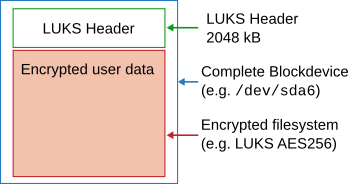
\includegraphics{luks.png}
				\caption{Esquema de \textit{LUKS}}
			\end{figure}
			Por tanto, deberemos crear ambos elementos manualmente.
			\item Lo primero que debemos hacer es entrar en modo de mantenimiento:
			\begin{lstlisting}[xleftmargin=-3.8cm]
				#> systemctl isolate runlevel1.target
			\end{lstlisting}
			\item Después creamos la cabecera dando el formato \textit{LUKS}. La sintaxis es la siguiente:
			\begin{lstlisting}[xleftmargin=-3.8cm]
				#> cryptsetup luksFormat <dispositivo>
			\end{lstlisting}
			En nuestro caso:
			\begin{lstlisting}[xleftmargin=-3.8cm]
				#> cryptsetup luksFormat /dev/pmraid1/newvar
			\end{lstlisting}
			Introducimos \textit{YES} (en mayúsculas) y establecemos la clave \textit{practicas,ISE}. Al ejecutar este comando borramos todos los datos del volumen.
			\item Ahora creamos el sistema de archivos encriptado:
			\begin{lstlisting}[xleftmargin=-3.9cm]
				#> cryptsetup luksOpen <dispositivo> <nombre del SA>
			\end{lstlisting}
			Que en nuestro caso sería:
			\begin{lstlisting}[xleftmargin=-3.8cm]
				#> cryptsetup luksOpen /dev/pmraid1/newvar pmraid1-newvar_crypt
			\end{lstlisting}
			Introducimos la clave anteriormente definida y comprobamos que se ha creado mediante \textit{lsblk}.
			\item Por último, modificamos el archivo \textit{/etc/crypttab}, que se encarga de asociar los volúmenes con formato \textit{LUKS} con sus respectivos sistemas de archivos cifrados. Su estructura es la siguiente:
			\begin{lstlisting}[xleftmargin=-3.8cm]
				<nombre del SA> UUID=<UUID del volumen LUKS> TYPE=none
			\end{lstlisting}
			El \textit{UUID, \textbf{U}niversal \textbf{U}nique \textbf{D}evice \textbf{ID}entifier} de un dispositivo es una forma de identificarlo unívocamente. Se obtiene mediante \textit{blkid}. Para no tener que copiarlo a mano, redirigimos la salida al archivo:
			\begin{lstlisting}[xleftmargin=-3.8cm]
				#> blkid | grep crypto >> /etc/crypttab
			\end{lstlisting}
			\item Ahora editamos el archivo mediante \textit{vi} y lo adaptamos a su formato. Debemos quitar las comillas del UUID. Debería quedar algo así:
			\begin{lstlisting}[xleftmargin=-3.8cm]
				pmraid1-newvar_crypt UUID=<UUID obtenido con grep sin comillas> TYPE=none
			\end{lstlisting}
	\end{enumerate}
	\item Continuamos como en la práctica 2. Damos formato al volumen encriptado:
	\begin{lstlisting}
		#> mkfs -t ext4 /dev/mapper/pmraid1-newvar_crypt
	\end{lstlisting}
	\item Montamos el SA:
	\begin{lstlisting}
		#> mkdir /mnt/varCifr
		#> mount /dev/mapper/pmraid1-newvar_crypt /mnt/varCifr
	\end{lstlisting}
	Comprobamos con \textit{mount}
	\item Copiamos los archivos:
	\begin{lstlisting}
		#> cp -a /var/. /mnt/varCifr
	\end{lstlisting}
	\item Editamos \textit{/etc/fstab} añadiendo la siguiente línea:
	\begin{lstlisting}
		/dev/mapper/pmraid1-newvar_crypt /var ext4 defaults 0 0
	\end{lstlisting}
	\item Desmontamos el volumen:
	\begin{lstlisting}
		#> umount /mnt/varCifr
	\end{lstlisting}
	Comprobamos con \textit{mount}.
	\item Borramos los datos antiguos:
	\begin{lstlisting}
		#> mv /var /varOld
	\end{lstlisting}
	En un tiempo prudencial se eliminaría el directorio \textit{/varOld}.
	\item Creamos \textit{/var} de nuevo:
	\begin{lstlisting}
		#> mkdir /var
	\end{lstlisting}
	\item Restauramos el contexto:
	\begin{lstlisting}
		#> restorecon /var
	\end{lstlisting}
	\item Montamos los sistemas de archivos de \textit{/etc/fstab}:
	\begin{lstlisting}
		#> mount -a
	\end{lstlisting}
	Comprobamos con \textit{mount}.
	\item Para finalizar, podemos ejecutar \textit{lsblk} para confirmar que todo está conforme al esquema.
	\item Reiniciamos la máquina y debería pedirnos la clave del cifrado.
	\item Tomamos una instantánea de la máquina.
\end{enumerate}

\subsubsection{Configuración de red de CentOS}
\begin{enumerate}
	\item Comenzamos añadiendo la interfaz de sólo anfitrión en el adaptador 2 de la máquina mediante VirtualBox (igual que en la sesión 1).
	\item Buscamos en qué interfaz se encuentra la nueva red. Para ello ejecutamos:
	\begin{lstlisting}
		$> ip addr
	\end{lstlisting}
	y vemos que la nueva es \textit{enp0s8}.
	\item Nos logueamos con permisos \textit{root} mediante \textit{su}
	\item Creamos su script de configuración:
	\begin{lstlisting}
		#> vi /etc/sysconfig/network-scripts/ifcfg-enp0s8
	\end{lstlisting}
	y añadimos el siguiente contenido:
	\begin{lstlisting}
		TYPE=Ethernet
		BOOTPROTO=none
		NAME=enp0s8
		DEVICE=enp0s8
		ONBOOT=yes
		IPADDR=192.168.56.110
		NETMASK=255.255.255.0
	\end{lstlisting}
	\item Levantamos la interfaz:
	\begin{lstlisting}
		#> ifup enp0s8
	\end{lstlisting}
	\item Podemos editar el archivo \textit{ifcfg-enp0s3} para activar el flag \textit{ONBOOT} y que la interfaz que nos conecta con Internet se active al iniciar:
	\begin{lstlisting}
		#> vi /etc/sysconfig/network-scripts/ifcfg-enp0s3
	\end{lstlisting}
	Cambiamos \textit{ONBOOT=no} por \textit{ONBOOT=yes}.
\end{enumerate}
Ahora comprobamos que toda la conectividad funciona. Para ello arrancamos ambas máquinas, CentOS y Ubuntu Server. Realizaremos las siguientes pruebas:
\begin{itemize}
	\item Ping entre las máquinas:
	\begin{lstlisting}
		Ubuntu Server $> ping 192.168.56.110 -c 5
		CentOS        $> ping 192.168.56.105 -c 5
	\end{lstlisting}
	\item Ping de las máquinas al host (actúa como router):
	\begin{lstlisting}
		 $> ping 192.168.56.1 -c 5
	\end{lstlisting}
	\item Ping desde el anfitrión a las máquinas:
	\begin{lstlisting}
	$> ping 192.168.56.105 -c 5
	$> ping 192.168.56.110 -c 5
	\end{lstlisting}
	\item Ping entre las máquinas e Internet:
	\begin{lstlisting}
	$> ping google.es -c 5
	\end{lstlisting}
\end{itemize}
En todos los casos las 5 respuestas deberían ser recibidas.\\

El esquema de red resultante es el siguiente:

\begin{figure}[H]
	\centering
	\begin{tikzpicture}[arrow/.style = {thick}, node distance=2cm]
		\tikzset{set/.style={draw,rectangle,inner sep=0pt,align=center}}

		% Host
		\node[diamond,fit={(0,0) (1,1)}, inner sep=0pt, draw=black, thick, text centered,align=center, fill=violet!20] (host) {Host};

		% Host connectors

		\node[rectangle, above of =host,node distance = 2cm,inner sep=0pt, draw=black, thick, text centered,fill=green!50, minimum width = 1.6cm, minimum height=1cm, node distance = 2.2cm] (vboxnet0) {\footnotesize vboxnet0};

		\node[rectangle, below of =host,node distance = 2.85cm,inner sep=0pt, draw=black, thick, text centered,fill=red!50, minimum size = 1cm] (hostnat) {\footnotesize NAT};

		% CentOS
		\node[circle, left of=host,node distance = 5cm, minimum size = 2cm,inner sep=0pt, draw=black, thick, text centered,fill=blue!30] (centos) {CentOS};


		\node[rectangle, below right of =centos,node distance = 4cm,inner sep=0pt, draw=black, thick, text centered,fill=blue!30, minimum size = 1cm] (centosnat) {\footnotesize NAT};
		\node[rectangle, above of =centosnat,node distance = 6.7cm,inner sep=0pt, draw=black, thick, text centered,fill=green!50, minimum size = 1cm] (centosho) {\footnotesize HO};


		% Ubuntu Server
		\node[circle, right of=host,node distance = 5cm, minimum size = 2cm,inner sep=0pt, draw=black, thick, text centered,fill=yellow!20, align=center] (ubuntu) {Ubuntu \\ Server};

		\node[rectangle, below left of =ubuntu,node distance = 4cm,inner sep=0pt, draw=black, thick, text centered,fill=yellow!20, minimum size = 1cm] (ubuntunat) {\footnotesize NAT};
		\node[rectangle, above of =ubuntunat,node distance = 6.7cm,inner sep=0pt, draw=black, thick, text centered,fill=green!50, minimum size = 1cm] (ubuntuho) {\footnotesize HO};



		% Internet
		\node[cloud, below of=hostnat,node distance = 3cm, minimum width=3cm,inner sep=0pt, draw=black, thick, text centered,fill=blue!10, align=center] (internet) {Internet};



		% Arrows

		\draw [arrow,draw=red] (host) -- (vboxnet0);
		\draw [arrow] (host) -- (hostnat);


		\draw [arrow] (centos) -- (centosho);
		\draw [arrow] (centos) -- (centosnat);

		\draw [arrow] (ubuntu) -- (ubuntuho);
		\draw [arrow] (ubuntu) -- (ubuntunat);

		\draw [arrow] (centosnat) -- (hostnat);
		\draw [arrow] (ubuntunat) -- (hostnat);

		\draw [arrow] (hostnat) -- (internet);

		\draw [arrow,draw=red] (ubuntuho) -- (centosho);
		\coordinate (hocenter) at ($(ubuntuho)!0.5!(centosho)$);
		\draw [arrow,draw=red] (hocenter) -- (vboxnet0);

		% IP addresses
		\node[above right of =ubuntu] {192.168.56.105};
		\node[above left of =centos] {192.168.56.110};
		\node[below right of =host, node distance = 1.7cm] {192.168.56.1};



	\end{tikzpicture}
\end{figure}

Añadimos la interfaz sólo anfitrión porque las máquinas no pueden comunicarse entre ellas mediante NAT.


\section{Práctica 2: Instalación y configuración de servicios}

\subsection{Sesión 1}

En esta sesión instalaremos el servicio \textit{ssh} en Ubuntu. SSH es un protocolo de administración remota que permite que otro se usuario se conecte a nuestro servidor y lo maneje (y viceversa). Consta de dos elementos:
\begin{itemize}
	\item \textit{\textbf{ssh}}. Es el cliente. Sirve para conectarnos a otra máquina.
	\item \textit{\textbf{sshd} (SSH Daemon)}. Es el servidor, sirve para que otras máquinas se conecten a la nuestra.
\end{itemize}


\begin{enumerate}
	\item Comenzamos arrancando la máquina en la instantánea de la instalación limpia con la red configurada.
	\item Instalamos el paquete mediante:
	\begin{lstlisting}
		$> sudo apt install openssh-server
	\end{lstlisting}
	\item Si ejecutamos \textit{systemctl status ssh} podemos ver que el servicio está activo y que su PID cuelga del servidor (\textit{sshd}). Es decir, Ubuntu, a diferencia de CentOS, no diferencia entre \textit{ssh} y \textit{sshd}.
	\item Para poder conectarnos por SSH a una máquina debemos ejecutar el comando:
	\begin{lstlisting}
		$> ssh IP -l usuario (-p puerto)
	\end{lstlisting}
	El usuario por defecto es el de la sesión abierta en ese momento y el puerto el 22.
	Probamos a ejecutarlo desde el host:
	\begin{lstlisting}
		Host $> ssh 192.168.56.105 -l csp
	\end{lstlisting}
	Si en alguna ocasión nos hemos conectado a esa máquina mediante SSH, tendremos que eliminar el correspondiente contenido de \textit{\~{}/.ssh/known\_hosts} mediante
	\begin{lstlisting}
		Host $> ssh-keygen -f "~/.ssh/known_hosts" -R "192.168.56.105"
	\end{lstlisting}


	\item Vamos a cambiar varios parámetros del \textbf{servidor}. Para ello editamos su archivo de configuración:
	\begin{lstlisting}
		$> sudo vi /etc/ssh/sshd_config
	\end{lstlisting}
	\begin{itemize}
		\item Cambiamos el puerto al 22022 cambiando la línea
		\begin{lstlisting}
			PORT 22
		\end{lstlisting}
		por
		\begin{lstlisting}
			PORT 22022
		\end{lstlisting}
		\item Desactivamos el acceso root cambiando la línea
		\begin{lstlisting}
			PermitRootLogin prohibit-password
		\end{lstlisting}
		por
		\begin{lstlisting}
			PermitRootLogin no
		\end{lstlisting}
	\end{itemize}
	Para que los cambios hagan efecto reiniciamos el servicio mediante
	\begin{lstlisting}
		$> sudo systemctl restart sshd
	\end{lstlisting}
	Podemos comprobar que los cambios han funcionado conectándonos desde el host con el nuevo puerto o mediante \textit{systemctl status sshd}.
	\item Pasamos a crear la clave público privada. Se trata de un paradigma en el que el cliente genera una llave (clave privada) y un candado (clave pública), que es entregado al servidor. Para autenticarse, el cliente enviará su llave y si encaja con el candado, recibirá acceso. En nuestro caso, el cliente será CentOS y el servidor Ubuntu.
	\begin{enumerate}
		\item Comenzamos creando llave y candado en CentOS:
		\begin{lstlisting}
		CentOS $> ssh-keygen
		\end{lstlisting}
		Pulsamos Enter tres veces para elegir el destino por defecto y no establecer contraseña. Vemos que se crean dos archivos: \textit{id\_rsa} (clave privada, llave) e \textit{id\_rsa.pub} (clave pública, candado).
		\item Entregamos la clave pública al servidor mediante:
		\begin{lstlisting}
		CentOS $> ssh-copy-id 192.168.56.105 -p 22022
		\end{lstlisting}
		Introducimos la clave y pulsamos Enter.
		\item Comprobamos que todo ha ido bien conectándonos:
		\begin{lstlisting}
		CentOS $> ssh 192.168.56.105 -p 22022
		\end{lstlisting}
	\end{enumerate}
\end{enumerate}

\begin{figure}[H]
	\centering
	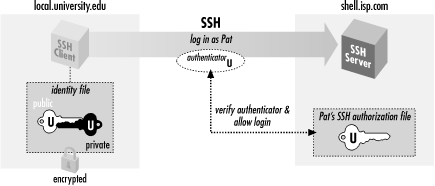
\includegraphics[width=0.9\textwidth]{sshrsa.png}
	\caption{Esquema clave público-privada en SSH}
\end{figure}

\subsection{Sesión 2}

En esta sesión instalaremos el servicio SSH en CentOS y veremos las diferencias que hay con respecto a Ubuntu.

\begin{enumerate}
	\item Primero comprobamos si el servicio está instalado:
	\begin{lstlisting}
		$> systemctl status sshd
	\end{lstlisting}
	Podemos ver que sí que está activo. Sin embargo, no se nos muestra el puerto porque no somos usuarios root. Nos logueamos mediante \textit{su} y ejecutamos de nuevo el comando anterior. Veremos que el puerto es el predeterminado (22).
	\item Accedemos a la cofiguración para editar tanto el acceso root como el puerto:
	\begin{lstlisting}
		#> vi /etc/ssh/sshd_config
	\end{lstlisting}
	Vemos que todo el archivo está comentado. Para modificar las reglas, descomentamos y editamos las líneas correspondientes:
	\begin{lstlisting}
			Port 22022
			PermitRootLogin no
	\end{lstlisting}
	Vemos que encima de la regla del puerto se nos especifica que tenemos que informar a SELinux del cambio que hemos realizado mediante \textit{semanage}, que no está instalado por defecto.
	\item Buscamos el paquete que incluye la herramienta \textit{semanage}:
	\begin{lstlisting}
		#> yum provides semanage
	\end{lstlisting}
	Instalamos el paquete que recibimos como respuesta:
	\begin{lstlisting}
		#> yum install -y policycoreutils-python-2.5-33.el7.x86_64
	\end{lstlisting}
	\item Configuramos el puerto:
	\begin{lstlisting}
		#> semanage port -a -t ssh_port_t -p tcp 22022
	\end{lstlisting}
	Comprobamos que la regla se añadió mediante:
	\begin{lstlisting}
		#> semanage port -l | grep ssh
	\end{lstlisting}
	\item Ya tenemos \textit{sshd} configurado y se puede acceder desde el equipo local. Sin embargo, debemos añadir una regla al firewall que permita las conexiones entrantes para el servicio (por defecto las bloquea).
	\begin{lstlisting}
		#> firewall-cmd --permanent --add-port=22022/tcp
	\end{lstlisting}
	\item Finalmente, reiniciamos los servicios:
	\begin{lstlisting}
		#> firewall-cmd --reload
		#> systemctl restart sshd
	\end{lstlisting}
\end{enumerate}

En Ubuntu el firewall se denomina \textit{ufw}. Sus comandos principales son:
\begin{lstlisting}
	$> sudo ufw enable							# Activar
	$> sudo ufw disable						# Desactivar
	$> sudo ufw allow <port>	# Nueva regla
\end{lstlisting}

Podemos sintetizar las diferencias entre Ubuntu y CentOS en la siguiente tabla:
\begin{figure}[H]
	\centering
	\begin{tabular}{|m{1.4cm}|m{2cm}|m{2.2cm}|m{2.2cm}|m{3cm}|m{1.5cm}|}
		\hline
		 	SO & Activo por defecto & Nombre del servidor & Archivo de configuración & Acceso root por defecto & Firewall \\
		 \hline
		 Ubuntu & \textcolor{red}{$\times$} & SSH,SSHD & Sin comentar & \textcolor{red}{$\times$} (prohibit-password) & UFW. Desactivado por defecto \\
		 \hline
		 CentOS & \greencheck & SSHD & Comentado & \greencheck & firewall-cmd. Activado por defecto.\\
		 \hline

	\end{tabular}
\end{figure}

\subsection{Sesión 3}
En esta sesión instalaremos la pila LAMP (Linux, Apache, MySQL, PHP) en Ubuntu y CentOS.
Comencemos con Ubuntu:

\begin{enumerate}
  \item Abrimos el instalador gráfico de paquetes:
  \begin{lstlisting}
  	$> sudo tasksel
  \end{lstlisting}
  \item Seleccionamos \textit{LAMP Server} con la barra espaciadora y pulsamos Enter.
  \item Establecemos la contraseña root de MySQL (\textit{practicas,ISE}).
  \item Esperamos a que termine de instalar y probamos los componentes uno a uno:
  \begin{enumerate}
    \item Apache: ejecutamos \textit{curl localhost} o visitamos \textit{192.168.56.105} desde el navegador del host y confirmamos que podemos ver la página por defecto de Apache.
    \item MySQL: ejecutamos \textit{mysql -u root -p}, introducimos la clave del root y comprobamos que tenemos acceso al servidor mediante el cliente (la consola).
    \item PHP: ejecutamos \textit{php -a} y accedemos a la consola. Podemos comprobar que todo va bien ejecutando \textit{echo("Prueba");}
  \end{enumerate}
\end{enumerate}

  Ya estaría terminada la instalación en Ubuntu. Vamos ahora a CentOS:
  \begin{enumerate}
    \item Nos logueamos como superusuario mediante \textit{su}.
    \item Comenzamos instalando Apache, que en CentOS se llama \textit{httpd}:
    \begin{lstlisting}
      #> yum install -y httpd
    \end{lstlisting}
    \item Vemos si el servicio está activado e iniciado:
    \begin{lstlisting}
      #> systemctl status httpd
    \end{lstlisting}
    \item Vemos que tenemos que hacer ambas cosas:
    \begin{lstlisting}
      #> systemctl enable httpd
      #> systemctl start httpd
    \end{lstlisting}
    \item Comprobamos que el servicio funciona:
    \begin{lstlisting}
      #> curl localhost
    \end{lstlisting}
    \item Tenemos el servicio en ejecución y funcionando, pero no podemos acceder desde otra máquina. Añadimos la correspondiente regla permanente al firewall y lo reiniciamos para que se aplique:
    \begin{lstlisting}
      #> firewall-cmd --permanent --add-port=80/tcp
      #> firewall-cmd --reload
    \end{lstlisting}
    Por último, comprobamos que ya podemos acceder desde el host.
    \item Pasamos a instalar MySQL. En CentOS instalaremos la versión gratuita (MariaDB).
    \begin{lstlisting}
      #> yum install -y mariadb-server
    \end{lstlisting}
    \item Comprobamos el estado del servicio:
    \begin{lstlisting}
      #> systemctl status mariadb
    \end{lstlisting}
    y lo habilitamos e iniciamos:
    \begin{lstlisting}
      #> systemctl enable mariadb
      #> systemctl start mariadb
    \end{lstlisting}
    \item Configuramos el usuario root mediante el comando \textit{mysql\_secure\_installation} (damos YES a todo).
    \item Accedemos a la consola con \textit{mysql -u root -p} y creamos una nueva base de datos.
    \begin{lstlisting}
      MariaDB > create database mi_bd;
    \end{lstlisting}
    \item Pasamos a PHP. Lo instalamos:
    \begin{lstlisting}
      #> yum install php -y
    \end{lstlisting}
    y probamos que funciona (igual que en Ubuntu).
    \item Ya tenemos la pila LAMP instalada. Ahora vamos a comprobar si podemos enlazar los componentes entre sí. La idea es montar un script PHP que acceda a la base de datos \textit{mi\_bd} y ejecutarlo desde el servidor web. Comenzamos instalando el conector:
    \begin{lstlisting}
      #> yum install -y php-mysql
    \end{lstlisting}
    \item Ahora creamos el script:
    \begin{lstlisting}
      #> vi /var/www/html/miscript.php
    \end{lstlisting}
    \item Accedemos a \href{https://www.php.net/manual/es/function.mysqli-connect.php}{esta} web y copiamos el ejemplo en vi. Modificamos el usuario y la contraseña con \textit{root} y \textit{practicas,ISE} respectivamente.
    \item Ejecutamos el script para ver que funciona:
    \begin{lstlisting}
      #> php /var/www/html/miscript.php
    \end{lstlisting}
    \item Ahora intentamos acceder a la ruta del archivo (\textit{192.168.56.110/miscript.php}) desde el host y vemos que el script no se ha ejecutado, sino que estamos viendo el contenido. Accedemos a la configuración del servidor para arreglar esto:
    \begin{lstlisting}
      #> vi /etc/httpd/conf/httpd.conf
    \end{lstlisting}
    Cambiamos el texto
    \begin{lstlisting}
    <IfModule dir_module>
      DirectoryIndex index.html
    </IfModule>
    \end{lstlisting}
    por
    \begin{lstlisting}
    <IfModule dir_module>
      DirectoryIndex index.html miscript.php
    </IfModule>
    \end{lstlisting}
    \item Reiniciamos el servicio y comprobamos si funciona:
    \begin{lstlisting}
      #> systemctl restart httpd
    \end{lstlisting}
    \item Vemos que ya si que se nos ejecuta, pero la conexión no se realiza. Debemos autorizarla a través de SELinux:
    \begin{lstlisting}
      #> setsebool -P httpd_can_network_connect_db 1
    \end{lstlisting}
    \item Probamos ahora y vemos que funciona correctamente.
\end{enumerate}

\subsubsection{Screen}

Screen es una utilidad que permite crear sesiones de shell que podemos "descolgar" de la shell principal. Esto es muy útil si dejamos algún proceso ejecutando y la sesión se cierra.\\
El comando para instalar la herramienta es:

\begin{lstlisting}
          #> yum install -y screen
\end{lstlisting}

Los comandos más útiles son:
\begin{enumerate}
  \item screen: crea una nueva sesión. Para descolgarla debemos pulsar Ctrl+A+D.
  \item screen -list: ver una lista de las sesiones abiertas junto con su PID.
  \item screen -r $<pid>$: permite recuperar la sesión asociada a $<pid>$.
  \item exit: permite cerrar una sesión.
\end{enumerate}

  Vamos a ver dos herramientas interesantes: \textit{Fail2Ban} y \textit{RKHunter}. Ambas herramientas se encuentran en la release \textit{EPEL (Extra Packages Enterprise Linux)}, por lo que deberemos instalar primero la release con:
  \begin{lstlisting}
    #> yum install -y epel-release
  \end{lstlisting}


  \subsubsection{Fail2Ban}

  Fail2Ban es una herramienta que se encarga de "banear" las IPs que intenten acceder a nuestra máquina y fallen más de $n$ veces (por defecto 5).

  \begin{enumerate}
    \item Comenzamos instalando la utilidad:
    \begin{lstlisting}
      #> yum install -y fail2ban
    \end{lstlisting}
    \item Activamos e iniciamos el servicio:
    \begin{lstlisting}
      #> systemctl enable fail2ban
      #> systemctl start fail2ban
    \end{lstlisting}
    \item Podemos ver el estado del servicio mediante
    \begin{lstlisting}
      #> fail2ban-client status
    \end{lstlisting}
    \item Vamos a configurar una \textit{jail} que baneará a los usuarios que introduzcan erróneamente sus credenciales en el servicio SSH. Comenzamos creando una copia del archivo de configuración (fail2ban toma los archivos \textit{.local} como configuración, no el \textit{.conf}).
    \begin{lstlisting}
      #> cd /etc/fail2ban
      #> cp jail.conf jail.local
    \end{lstlisting}
    \item Editamos el archivo de configuración:
    \begin{lstlisting}
      #> vi jail.local
    \end{lstlisting}
    \item Vamos a la jail de SSH:
    \begin{lstlisting}
      # JAILS
      [sshd]
    \end{lstlisting}
    y añadimos lo siguiente bajo \textit{[sshd]}
    \begin{lstlisting}
      # JAILS
      [sshd]
      enabled=true
      port=22022
    \end{lstlisting}
    \item Reiniciamos el servicio y comprobamos que la cárcel funciona intentando acceder a ssh desde el host y fallando 5 veces.
    \item Desbaneamos al host mediante:
    \begin{lstlisting}
      #> fail2ban-client set sshd unban 192.168.56.1
    \end{lstlisting}
  \end{enumerate}

  \subsubsection{RKHunter}

  RKHunter (\textit{RootKit Hunter}) es una herramienta que escanea nuestro sistema en busca de amenazas como rootkits, troyanos, etc. Se instala mediante
  \begin{lstlisting}
            #> yum install -y rkhunter
  \end{lstlisting}
y se ejecuta un análisis con
\begin{lstlisting}
            #> rkhunter -c
\end{lstlisting}



\section{Práctica 3: Monitorización y profiling}

\subsection{Sesión 1}

\subsection{Sesión 2}
En esta sesión instalaremos Zabbix en Ubuntu y lo configuraremos para que se monitorice a sí mismo y para que monitorice a CentOS. La documentación que usaremos será \href{https://www.zabbix.com/documentation/3.4/manual}{la siguiente}.\\

La idea es instalar \textit{server, frontend} y \textit{agent} en Ubuntu y \textit{agent} en CentOS. Veamos primero qué es cada componente:

\begin{itemize}
  \item \textbf{Server}. Es el proceso central del monitor. Se encarga de capturar información y enviarla a los usuarios.
  \item \textbf{Agent}. Monitoriza activamente los recursos y aplicaciones locales. Toma estos datos y los envía al servidor para que los procese.
  \item \textbf{Frontend}. Muestra los datos que se han tomado de forma gráfica.
\end{itemize}

\subsubsection{Instalación en Ubuntu}

\begin{enumerate}
  \item Arrancamos Ubuntu.
  \item Descargamos e instalamos el repositorio de Zabbix para nuestra versión de Ubuntu (Xenial):
  \begin{lstlisting}
  $> wget https://repo.zabbix.com/zabbix/3.4/ubuntu/pool/main/z/zabbix-release/zabbix-release_3.4-1+xenial_all.deb
  $> sudo dpkg -i zabbix-release_3.4-1+xenial_all.deb
  $> sudo apt update
  \end{lstlisting}
  \item Instalamos el servidor que funciona con MySQL y el frontend:
  \begin{lstlisting}
  $> sudo apt install -y zabbix-server-mysql zabbix-frontend-php
  \end{lstlisting}
  \item Pasamos ahora a la configuración de la base de datos. Comenzamos accediendo a MySQL y creando una nueva base de datos:
  \begin{lstlisting}
  $> mysql -u root -p
  mysql> create database zabbix character set utf8 collate utf8_bin;
  mysql> grant all privileges on zabbix.* to zabbix@localhost identified by 'practicas,ISE';
  mysql> exit;
  \end{lstlisting}
  \item Importamos el esquema inicial (el proceso tarda mucho, alrededor de media hora):
  \begin{lstlisting}
  $> zcat /usr/share/doc/zabbix-server-mysql/create.sql.gz | mysql -u zabbix -p zabbix
  \end{lstlisting}
  \item Accedemos al fichero de configuración:
  \begin{lstlisting}
  $> sudo vi /etc/zabbix/zabbix_server.conf
  \end{lstlisting}
  y establecemos la clave (el resto de campos vienen por defecto):
  \begin{lstlisting}
  DBPassword=practicas,ISE
  \end{lstlisting}
  \item Iniciamos y activamos el servicio:
  \begin{lstlisting}
  $> sudo systemctl enable zabbix-server
  $> sudo systemctl start zabbix-server
  \end{lstlisting}
  \item Configuramos la zona horaria de PHP:
  \begin{lstlisting}
  $> sudo vi /etc/php/7.0/apache2/php.ini
  \end{lstlisting}
  Buscamos el texto [Date] y lo modificamos:
  \begin{lstlisting}
  [Date]
  date.timezone="Europe/Madrid"
  \end{lstlisting}
  \item Reiniciamos el servidor web:
  \begin{lstlisting}
  $> sudo systemctl restart apache2
  \end{lstlisting}
  \item Añadimos la correspondiente regla al firewall:
  \begin{lstlisting}
  $> sudo ufw allow 80/tcp
  \end{lstlisting}
  \item Desde el host, accedemos  a \textit{192.168.56.105/zabbix} para iniciar el proceso de instalación. Pulsamos en \textit{Next} y deberíamos ver todos los flags en OK.
  \item Pasamos al siguiente paso e introducimos la contraseña de la base de datos en el campo \textit{Password}.
  \item Damos un nombre al servidor, por ejemplo, \textit{ZabbixUbuntu}.
  \item Revisamos todos los cambios y los aceptamos.
  \item Accedemos a la interfaz del frontend con las credenciales por defecto: Admin/zabbix.
  \item Por último, instalamos, activamos y arrancamos el agente:
  \begin{lstlisting}
  $> sudo apt install -y zabbix-agent
  $> sudo systemctl enable zabbix-agent
  $> sudo systemctl start zabbix-agent
  \end{lstlisting}

\end{enumerate}

\subsubsection{Instalación en CentOS}

Ahora instalaremos el agente en CentOS.

\begin{enumerate}
  \item Comenzamos logueándonos como root y añadiendo el repositorio:
  \begin{lstlisting}
  #> rpm -ivh https://repo.zabbix.com/zabbix/3.4/rhel/7/x86_64/zabbix-release-3.4-2.el7.noarch.rpm
  \end{lstlisting}
  \item Instalamos el agente:
  \begin{lstlisting}
  #> yum install -y zabbix-agent
  \end{lstlisting}
  \item Activamos y arrancamos el servicio:
  \begin{lstlisting}
  #> systemctl enable zabbix-agent
  #> systemctl start zabbix-agent
  \end{lstlisting}
  \item Vemos que al iniciar el servicio obtenemos un error relacionado con un límite de recursos. Para solucionarlo hacemos lo siguiente:
  \begin{lstlisting}
  #> cat /var/log/audit/audit.log | grep zabbix_agentd | grep denied | audit2allow -M zabbix_agent_setrlimit
  #> semodule -i zabbix_agent_setrlimit
  \end{lstlisting}
  \item Reiniciamos el servicio y vemos que ya no tenemos errores:
  \begin{lstlisting}
  #> systemctl restart zabbix-agent.pp
  \end{lstlisting}
  \item Añadimos la IP del servidor de Zabbix (Ubuntu) al archivo de configuración:
  \begin{lstlisting}
  #> vi /etc/zabbix/zabbix_agentd.conf
  \end{lstlisting}
  \begin{lstlisting}
  Server=192.168.56.105
  \end{lstlisting}
  \item Vemos que el puerto en el que escucha el agente es el 10500, por lo que debemos abrirlo tanto en CentOS como en Ubuntu:
  \begin{lstlisting}
  Ubuntu $> sudo ufw allow 10050/tcp
  CentOS #> firewall-cmd --zone=public --add-port=10050/tcp --permanent
  CentOS #> firewall-cmd --reload
  \end{lstlisting}
\end{enumerate}

\subsubsection{Añadir CentOS al frontend}

Ahora añadiremos el host CentOS al frontend. Para ello, accedemos a la web, Configurateion, Hosts, Create Host. Establecemos su nombre e IP:
\begin{lstlisting}
    Host name: CentOS
    New group: ISE
    IP address: 192.168.56.110
\end{lstlisting}

Para finalizar, activamos la monitorización de Ubuntu haciendo click en su estado (\textit{Disabled}).

\subsubsection{Monitorización de SSH y HTTP}

\begin{enumerate}
  \item Hacemos click en el host de CentOS que acabamos de crear.
  \item Vamos a la pestaña \textit{Templates}.
  \item Añadimos las siguientes plantillas:
  \begin{itemize}
    \item Template App HTTP Service
    \item Template App SSH Service
  \end{itemize}
  \item Pulsamos en \textit{Add} y luego en \textit{Update}.
  \item Debemos informar a la plantilla de SSH que servimos en el puerto 22022. Para ello, vamos a Configuration-Templates-Template App SSH Service.
  \item Vamos a Items-SSH service is running.
  \item En el campo \textit{Key} cambiamos
  \begin{lstlisting}
      net.tcp.service[ssh]
  \end{lstlisting}
  por
  \begin{lstlisting}
      net.tcp.service[ssh,,22022]
  \end{lstlisting}
  \item Hacemos click en \textit{Update} y reabrimos el frontend. Vemos que se nos marca el problema de conexión a SSH como resuelto en la pestaña \textit{Dashboard}.
\end{enumerate}





\newpage
\section{Preguntas de examen}
\subsection{Práctica 1}
\begin{enumerate}
  \item Si monto un RAID0 y un RAID1 con 2 HDD de 10GB, ¿cuánto espacio tengo disponible?
  \begin{solution}
    \begin{itemize}
      \item RAID0: 20GB, ya que no hay redundancia.
      \item RAID1: 10GB, ya que los datos se replican.
    \end{itemize}
  \end{solution}
  ¿Y si uso un HDD de 10GB y otro de 50GB?
  \begin{solution}
    \begin{itemize}
      \item RAID0: 60GB.
      \item RAID1: 10GB. Si tomáramos más espacio no podría replicarse.
    \end{itemize}
  \end{solution}
  \item Disponemos de un sistema con particiones \textit{home}, \textit{swap}, \textit{boot} y \textit{root}. Sólo podemos encriptar una de ellas. ¿Cuál elegirías?
  \begin{solution}
    SWAP, ya que contiene datos de la RAM, como claves, archivos de las aplicaciones, etc.
  \end{solution}
	\item ¿Qué diferencias hay entre \textit{EXT2} y \textit{EXT4}?
	\begin{solution}
		\textit{EXT4}, a diferencia de \textit{EXT2}, admite \textit{journaling}, es decir, un diario que permite restablecer los datos anteriores a una transacción en caso de que ésta falle. Esta técnica permite al sistema de archivos volver a un estado coherente si se produce un corte de electricidad o cualquier otro fallo durante una transacción. Otra característica muy interesante de \textit{EXT4} es el asignamiento multi-bloque, que permite asignar varios bloques en una misma llamada.
	\end{solution}
	\item ¿Qué diferencias hay entre:
	\begin{itemize}
		\item \textit{cp -a /var/ /newvar}
		\item \textit{cp -a /var/* /newvar}
		\item \textit{cp -a /var/. /newvar}
	\end{itemize}
	?
	\begin{solution}
		\begin{itemize}
			\item \textit{cp -a /var /newvar} copia la carpeta, no el contenido. Es decir, quedaría \textit{/newvar/var/archivos}
			\item \textit{cp -a /var/* /newvar} no copia los archivos ocultos.
			\item \textit{cp -a /var/. /newvar} copia todos los archivos (visibles y ocultos).
		\end{itemize}
	\end{solution}
	\item ¿Qué tipos de \textit{LUKS} hay? ¿Cuál usamos nosotros en la sesión 3 de la práctica 1?
	\begin{solution}
		\begin{itemize}
			\item \textit{LUKS} on \textit{LVM}. Consiste en montar la pila LVM y después cifrar mediante \textit{LUKS} los LV deseados. Es más eficiente y permite tener LV cifrados y LV no cifrados. Es el óptimo cuando no se quiere cifrar todo el disco.
			\item \textit{LVM} on \textit{LUKS}. Ciframos todo el disco con \textit{LUKS} y después montamos LVM encima. Es más seguro pero conlleva un peor rendimiento.
		\end{itemize}
		En la sesión 3 de la práctica 1 utilizamos \textit{LUKS} on \textit{LVM}.
	\end{solution}
\end{enumerate}

\newpage

\subsection{Práctica 2}

\begin{enumerate}
	\item Tras instalar el servicio \textit{ssh} en una máquina, ¿está activo?
	\begin{solution}
		Sí, está activo con los parámetros por defecto, por ejemplo, el puerto 22.
	\end{solution}
	\item ¿Cómo diferencia Ubuntu entre el cliente y el servidor SSH?
	\begin{solution}
		No lo hace, para él ambos son el mismo servicio (el PID de \textit{ssh} cuelga del de \textit{sshd}). Lo que sí debemos tener en cuenta es el archivo de configuración que editamos (\textit{/etc/ssh/sshd\_config} o \textit{/etc/ssh/ssh\_config}).
	\end{solution}
	\item ¿Hay algún problema si consiguen robarme la clave pública (candado)?
	\begin{solution}
		No, ya que solo la clave privada asociada (llave) es capaz de abrirlo. Lo que sí que sería un problema es que alguien obtuviera la clave privada, ya que podría acceder a la máquina con facilidad.
	\end{solution}
\end{enumerate}






\end{document}
